\documentclass[12pt, a4paper]{article}

% ─── Pacotes ──────────────────────────────────────────────────────────────────
\usepackage[utf8]{inputenc}
\usepackage[T1]{fontenc}
\usepackage[english]{babel}
\usepackage[top=3cm, bottom=2.5cm, left=3cm, right=2cm]{geometry}
\usepackage{graphicx}
\usepackage{tabularx}
\usepackage{longtable}
\usepackage{booktabs}
\usepackage{multirow}
\usepackage{array}
\usepackage{enumitem}
\usepackage{setspace}
\usepackage{indentfirst}
\usepackage{amsmath}
\usepackage{fancyhdr}
\usepackage{titlesec}
\usepackage{hyperref}
\usepackage{listings}
\usepackage{xcolor}
\usepackage{tcolorbox}
\usepackage{tikz}


\usetikzlibrary{shapes.geometric, arrows.meta, positioning, fit, backgrounds, calc, decorations.pathreplacing}
\tcbuselibrary{skins, breakable}

% ─── Cores ────────────────────────────────────────────────────────────────────
\definecolor{corPrimaria}{RGB}{83, 74, 183}
\definecolor{corTeal}{RGB}{15, 110, 86}
\definecolor{corCoral}{RGB}{153, 60, 29}
\definecolor{corAmber}{RGB}{133, 79, 11}
\definecolor{corCinza}{RGB}{80, 80, 80}
\definecolor{corFundoCodigo}{RGB}{248, 248, 248}
\definecolor{corComentario}{RGB}{60, 120, 60}
\definecolor{corChave}{RGB}{40, 40, 160}
\definecolor{corString}{RGB}{160, 40, 40}
\definecolor{corNumero}{RGB}{100, 60, 160}
\definecolor{corFundoInfo}{RGB}{230, 240, 255}
\definecolor{corBordaInfo}{RGB}{83, 74, 183}
\definecolor{corFundoAviso}{RGB}{255, 248, 225}
\definecolor{corBordaAviso}{RGB}{180, 120, 0}
\definecolor{corFundoAlerta}{RGB}{255, 236, 230}
\definecolor{corBordaAlerta}{RGB}{180, 60, 30}

% ─── Estilo de código ─────────────────────────────────────────────────────────
\lstdefinestyle{cpp}{
    language=C++,
    backgroundcolor=\color{corFundoCodigo},
    basicstyle=\ttfamily\footnotesize,
    keywordstyle=\color{corChave}\bfseries,
    commentstyle=\color{corComentario}\itshape,
    stringstyle=\color{corString},
    numberstyle=\tiny\color{corCinza},
    breaklines=true,
    frame=single,
    framerule=0.4pt,
    numbers=left,
    numbersep=6pt,
    showstringspaces=false,
    tabsize=2,
    captionpos=b,
    morekeywords={uint32_t, uint8_t, int16_t, bool, String, const}
}

\lstdefinestyle{python}{
    language=Python,
    backgroundcolor=\color{corFundoCodigo},
    basicstyle=\ttfamily\footnotesize,
    keywordstyle=\color{corChave}\bfseries,
    commentstyle=\color{corComentario}\itshape,
    stringstyle=\color{corString},
    numberstyle=\tiny\color{corCinza},
    breaklines=true,
    frame=single,
    framerule=0.4pt,
    numbers=left,
    numbersep=6pt,
    showstringspaces=false,
    tabsize=4,
    captionpos=b
}

\lstdefinestyle{bash}{
    backgroundcolor=\color{corFundoCodigo},
    basicstyle=\ttfamily\footnotesize\color{corCinza},
    breaklines=true,
    frame=single,
    framerule=0.4pt,
    showstringspaces=false
}

% ─── Caixas de destaque ───────────────────────────────────────────────────────
\tcbset{
    caixaInfo/.style={
        enhanced, breakable,
        colback=corFundoInfo, colframe=corBordaInfo,
        boxrule=0.8pt, arc=4pt,
        left=8pt, right=8pt, top=5pt, bottom=5pt,
        fonttitle=\bfseries\small\color{corBordaInfo},
        attach boxed title to top left={yshift=-2mm, xshift=4mm},
        boxed title style={colback=corBordaInfo, colframe=corBordaInfo, arc=2pt}
    },
    caixaAviso/.style={
        enhanced, breakable,
        colback=corFundoAviso, colframe=corBordaAviso,
        boxrule=0.8pt, arc=4pt,
        left=8pt, right=8pt, top=5pt, bottom=5pt,
        fonttitle=\bfseries\small\color{corBordaAviso},
        attach boxed title to top left={yshift=-2mm, xshift=4mm},
        boxed title style={colback=corBordaAviso, colframe=corBordaAviso, arc=2pt}
    },
    caixaAlerta/.style={
        enhanced, breakable,
        colback=corFundoAlerta, colframe=corBordaAlerta,
        boxrule=0.8pt, arc=4pt,
        left=8pt, right=8pt, top=5pt, bottom=5pt,
        fonttitle=\bfseries\small\color{corBordaAlerta},
        attach boxed title to top left={yshift=-2mm, xshift=4mm},
        boxed title style={colback=corBordaAlerta, colframe=corBordaAlerta, arc=2pt}
    }
}

% ─── Seções ───────────────────────────────────────────────────────────────────
\titleformat{\section}
    {\large\bfseries\color{corPrimaria}}
    {\thesection}{0.8em}{}[\vspace{-0.3em}\textcolor{corPrimaria}{\rule{\linewidth}{0.6pt}}]

\titleformat{\subsection}
    {\normalsize\bfseries\color{corCinza}}
    {\thesubsection}{0.8em}{}

\titleformat{\subsubsection}
    {\normalsize\bfseries}
    {\thesubsubsection}{0.8em}{}

% ─── Cabeçalho/rodapé ─────────────────────────────────────────────────────────
\pagestyle{fancy}
\fancyhf{}
\fancyhead[L]{\small\color{corCinza}Projeto Integrador --- Microcontroladores}
\fancyhead[R]{\small\color{corCinza}Diagnóstico de Saúde de Transformadores}
\fancyfoot[C]{\small\thepage}
\renewcommand{\headrulewidth}{0.4pt}
\renewcommand{\footrulewidth}{0pt}

% ─── Espaçamento ──────────────────────────────────────────────────────────────
\onehalfspacing
\setlength{\parindent}{1.25cm}

% ─── Hyperref ─────────────────────────────────────────────────────────────────
\hypersetup{
    colorlinks=true,
    linkcolor=corPrimaria,
    urlcolor=corTeal,
    citecolor=corCinza,
    pdfauthor={Equipe Projeto Integrador},
    pdftitle={Sistema de Diagnóstico de Saúde de Transformadores}
}

% ══════════════════════════════════════════════════════════════════════════════
\begin{document}

% ─── Capa ─────────────────────────────────────────────────────────────────────
\begin{titlepage}
    \centering
    \vspace*{1.5cm}

    {\Large\bfseries\color{corPrimaria}
        SISTEMA DE DIAGNÓSTICO DE SAÚDE\\[0.4cm]
        DE TRANSFORMADORES ELÉTRICOS\\[0.3cm]
    }

    {\normalsize\color{corCinza}
        Projeto Integrador --- Microcontroladores\\
        Tema 2: Manutenção Preditiva e Diagnóstico Operacional via IoT\\[2.5cm]
    }

    \begin{tcolorbox}[caixaInfo, title={Equipe de Desenvolvimento}, width=10cm]
        \begin{center}
        \begin{tabular}{ll}
            \textbf{P1} & Hardware \& Condicionamento de Sinal \\[2pt]
            \textbf{P2} & Firmware Base (Sensores \& Tempo Real) \\[2pt]
            \textbf{P3} & DSP \& Algoritmos de Análise \\[2pt]
            \textbf{P4} & Comunicação IoT (MQTT \& WiFi) \\[2pt]
            \textbf{P5} & IHM Python (Dashboard \& Alertas) \\[2pt]
            \textbf{P6} & Diagnóstico, Relatórios \& Docs \\
        \end{tabular}
        \end{center}
    \end{tcolorbox}

    \vfill

    {\normalsize São Luís, Maranhão --- 2025}
\end{titlepage}

% ─── Sumário ──────────────────────────────────────────────────────────────────
\tableofcontents
\newpage

% ══════════════════════════════════════════════════════════════════════════════
\section{Introdução e Motivação}

\subsection{Contextualização}

Transformadores são componentes críticos em qualquer instalação elétrica industrial ou comercial. Uma falha não detectada num transformador pode resultar em interrupção de produção, danos irreversíveis a equipamentos conectados e riscos de incêndio por arco elétrico. No Brasil, a manutenção corretiva (consertar após a falha) ainda é a prática dominante em pequenas e médias instalações, em grande parte por falta de instrumentação acessível.

Sistemas comerciais de monitoramento contínuo de transformadores --- como os oferecidos por empresas como ABB, Siemens e Schneider Electric --- custam entre R\$~15.000 e R\$~80.000 por ponto de medição, tornando-os inviáveis para a maioria das aplicações. O presente projeto propõe uma alternativa de baixo custo, construída sobre hardware acessível (ESP32, sensores de menos de R\$~50,00 cada) com capacidade de comunicação IoT.

\subsection{Objetivos do Projeto}

O sistema a ser desenvolvido tem como objetivo central criar uma plataforma de \textbf{manutenção preditiva} para transformadores, capaz de:

\begin{itemize}[leftmargin=2cm]
    \item Monitorar continuamente as grandezas elétricas, térmicas e mecânicas do transformador;
    \item Detectar anomalias características de falhas em desenvolvimento (degradação de isolação, afrouxamento de núcleo, sobrecarga, curto entre espiras);
    \item Transmitir os dados em tempo real via protocolo MQTT para um painel de controle supervisório;
    \item Gerar alertas automáticos com sugestões de intervenção técnica;
    \item Registrar histórico com rastreabilidade por \emph{timestamp} para laudos técnicos.
\end{itemize}

\begin{tcolorbox}[caixaInfo, title={Por que isso importa?}]
A norma ABNT NBR 5356 e as diretrizes do IEEE C57 recomendam monitoramento contínuo de temperatura e corrente em transformadores de potência. Vibração anormal em 120~Hz e seus múltiplos indica diretamente afrouxamento das chapas do núcleo magnético (\emph{magnetostrição}), um fenômeno que aumenta progressivamente até causar falha catastrófica se não tratado.
\end{tcolorbox}

% ══════════════════════════════════════════════════════════════════════════════
\section{Fundamentação Teórica}

\subsection{Princípio de Funcionamento do Transformador}

Um transformador é um dispositivo eletromagnético que transfere energia elétrica entre dois circuitos isolados por meio de indução magnética mútua. Seus componentes essenciais são:

\begin{itemize}[leftmargin=2cm]
    \item \textbf{Bobina primária (N$_1$ espiras):} Conectada à rede de alimentação (220~V). A corrente alternada cria um campo magnético variável.
    \item \textbf{Núcleo de ferro laminado:} Conduz o fluxo magnético $\Phi$ gerado pelo primário até a bobina secundária com perdas mínimas. As chapas de aço-silício são laminadas justamente para reduzir correntes de Foucault.
    \item \textbf{Bobina secundária (N$_2$ espiras):} O fluxo magnético induz uma tensão proporcional à relação de espiras.
\end{itemize}

A relação fundamental que governa o transformador é:

\begin{equation}
    \frac{V_1}{V_2} = \frac{N_1}{N_2} = \frac{I_2}{I_1}
    \label{eq:transformador}
\end{equation}

\noindent\textbf{Variáveis da Equação~\ref{eq:transformador}:}
\begin{itemize}[leftmargin=3cm, itemsep=2pt, topsep=4pt]
    \item[$V_1$ (V)] Tensão eficaz aplicada ao enrolamento primário --- a tensão da rede elétrica (220~V);
    \item[$V_2$ (V)] Tensão eficaz induzida no enrolamento secundário --- a tensão de saída (12~V);
    \item[$N_1$]     Número de espiras do enrolamento primário (lado da rede);
    \item[$N_2$]     Número de espiras do enrolamento secundário (lado da carga);
    \item[$I_1$ (A)] Corrente eficaz que circula no enrolamento primário;
    \item[$I_2$ (A)] Corrente eficaz que circula no enrolamento secundário e é fornecida à carga.
\end{itemize}

\noindent A relação entre correntes aparece \emph{invertida} em relação à tensão: se o secundário tem menos espiras e portanto menor tensão, ele fornece uma corrente maior na mesma proporção --- a potência é conservada (descontadas as perdas). Matematicamente: se $V_2 = V_1/18{,}3$, então $I_2 = I_1 \times 18{,}3$. Para o transformador monitorado neste projeto (220~V / 12~V), a relação de espiras é $N_1/N_2 \approx 18{,}3$.

\subsection{Conceitos e Fenômenos Físicos Fundamentais}

Para compreender o que o sistema monitora e por que cada sensor está posicionado onde está, é necessário entender os fenômenos físicos que ocorrem dentro de um transformador em operação. Esta seção serve como referência rápida para todos os integrantes da equipe.

\subsubsection{Fluxo Magnético ($\Phi$)}

Quando uma corrente elétrica alternada circula pelo enrolamento primário, ela cria um campo magnético variável ao redor do fio. O núcleo de ferro laminado tem a função de \emph{concentrar e canalizar} esse campo até o enrolamento secundário, da mesma forma que um cano canaliza água. O fluxo magnético $\Phi$ (medido em Weber, Wb) é a grandeza que quantifica essa ``quantidade de campo'' que atravessa a seção transversal do núcleo.

A lei de Faraday estabelece que uma variação de fluxo no tempo induz uma tensão no secundário:
\begin{equation}
    e = -N_2 \cdot \frac{d\Phi}{dt}
    \label{eq:faraday}
\end{equation}

\noindent\textbf{Variáveis da Equação~\ref{eq:faraday}:}
\begin{itemize}[leftmargin=3cm, itemsep=2pt, topsep=4pt]
    \item[$e$ (V)]           Força eletromotriz (tensão) induzida no secundário;
    \item[$N_2$]             Número de espiras do enrolamento secundário;
    \item[$d\Phi/dt$ (Wb/s)] Taxa de variação do fluxo magnético no tempo;
    \item[``$-$'']           Sinal negativo: a tensão induzida se opõe à variação que a causou (Lei de Lenz).
\end{itemize}

\noindent Em outras palavras: sem variação de fluxo, não há tensão induzida. É por isso que transformadores só funcionam com corrente \emph{alternada} --- em corrente contínua o fluxo seria constante ($d\Phi/dt = 0$) e nada seria induzido no secundário.

\subsubsection{Saturação Magnética}

O núcleo de ferro não consegue conduzir fluxo magnético indefinidamente. Existe um limite físico chamado \textbf{saturação magnética}: acima de certo nível de campo aplicado ($H$), os domínios magnéticos do material já estão todos alinhados e o ferro simplesmente para de responder ao aumento de corrente.

Na prática, isso significa que:
\begin{itemize}[leftmargin=2cm]
    \item Abaixo da saturação: a relação entre corrente primária e fluxo é \emph{linear}. O transformador funciona normalmente.
    \item Na saturação: o fluxo ``trava'' enquanto a corrente continua subindo sem limite. O resultado é um pico de corrente massivo no primário sem correspondência no secundário.
\end{itemize}

\begin{tcolorbox}[caixaAviso, title={Por que a saturação importa para o diagnóstico?}]
Um transformador saudável, ao ser energizado, entra brevemente em saturação e gera o pico de \emph{inrush} (ver Seção~\ref{subsec:inrush}) que decai suavemente em décimos de segundo. Se a saturação ocorre com \emph{pico mais alto do que esperado} ou com \emph{decaimento assimétrico}, isso indica degradação do núcleo ou falha na isolação primária. O SCT-013 no primário captura exatamente esse evento.
\end{tcolorbox}

\subsubsection{Correntes de Foucault (Eddy Currents)}

O mesmo campo magnético variável que induz tensão no secundário também induz tensões no próprio núcleo de ferro. Como o ferro conduz eletricidade, essas tensões fazem circular correntes fechadas dentro do material --- as chamadas \textbf{correntes de Foucault} (ou \textit{eddy currents}). Essas correntes não fazem nenhum trabalho útil: elas apenas dissipam energia na forma de calor dentro do núcleo (\textbf{perdas no ferro}).

Para minimizá-las, o núcleo não é um bloco sólido de ferro, mas sim um empilhamento de \textbf{chapas finas isoladas entre si} (as lâminas de aço-silício). Ao dividir o núcleo em fatias, o caminho das correntes de Foucault é interrompido, reduzindo drasticamente as perdas.

\begin{tcolorbox}[caixaInfo, title={Conexão com o MPU6050}]
Quando as chapas do núcleo se afrouxam por vibração ou degradação do verniz isolante, as correntes de Foucault aumentam \emph{e} a amplitude de vibração em 120~Hz cresce. O MPU6050 detecta esse aumento de amplitude --- é o sinal diagnóstico de que as chapas precisam de aperto mecânico.
\end{tcolorbox}

\subsubsection{Histerese Magnética}

O núcleo de ferro não ``esquece'' instantaneamente o campo que recebeu. Quando a corrente primária inverte de sentido, o fluxo magnético não acompanha imediatamente --- existe um atraso chamado \textbf{histerese}. A energia gasta para vencer esse atraso a cada ciclo também se dissipa como calor no núcleo (perdas por histerese).

Em condições normais, as perdas por histerese são constantes e previsíveis para uma dada temperatura de operação. Um aumento anormal de temperatura \emph{sem} correspondente aumento de carga pode indicar que as propriedades magnéticas do núcleo degradaram (oxidação, temperatura excessiva prévia, envelhecimento), aumentando as perdas por histerese. O DS18B20 monitora exatamente essa variação térmica.

\subsubsection{Curto Parcial entre Espiras}

Uma das falhas mais perigosas e difíceis de detectar num transformador é o \textbf{curto parcial entre espiras adjacentes}: o verniz isolante que reveste o fio de cobre se degrada (por calor, vibração ou surtos de tensão), e algumas espiras entram em curto-circuito entre si, formando um ``loop'' de corrente fechado dentro da própria bobina.

Os efeitos são cumulativos e progressivos:
\begin{enumerate}[leftmargin=2cm]
    \item O número efetivo de espiras cai → a relação $N_1/N_2$ muda → a tensão de saída cai ligeiramente;
    \item O ``loop'' em curto dissipa potência como calor localizado → $\Delta T$ cresce;
    \item O aquecimento acelera a degradação do verniz vizinho → mais espiras entram em curto → ciclo destrutivo.
\end{enumerate}

\begin{tcolorbox}[caixaAlerta, title={Sinal Diagnóstico Combinado}]
O curto parcial entre espiras é detectado pela \textbf{combinação} de dois sinais: (1) gradiente térmico $\Delta T$ elevado para a carga atual, medido pelo DS18B20, e (2) queda na eficiência $\eta$, calculada pelos SCT-013. Nenhum dos dois sinais isolado é suficiente --- a correlação entre eles é o diagnóstico.
\end{tcolorbox}

\subsection{Fenômenos Diagnósticos Monitorados}
\label{sec:fenomenos}

\subsubsection{Corrente de Inrush}
\label{subsec:inrush}

Quando um transformador é conectado à rede elétrica pela primeira vez (ou após uma desconexão), o núcleo de ferro não possui fluxo magnético residual uniforme. Dependendo do instante exato em que a chave é fechada (a fase da onda de tensão naquele momento), o núcleo pode ser forçado a atingir um nível de fluxo que \emph{ultrapassa sua capacidade de saturação} nos primeiros semiciclos.

Como o núcleo saturado não oferece mais reatância (resistência ao fluxo), a corrente no primário sobe drasticamente limitada apenas pela resistência ôhmica do enrolamento --- que é baixíssima. Isso gera o chamado \textbf{inrush current}: um pico de corrente que pode atingir \textbf{8 a 12 vezes} a corrente nominal, com duração típica de 0,1 a 0,3 segundos, decaindo exponencialmente conforme o núcleo ``se magnetiza'' de forma estável.

A análise do perfil de inrush revela o estado do núcleo:

\begin{itemize}[leftmargin=2cm]
    \item \textbf{Inrush normal:} Pico elevado com decaimento exponencial suave --- o núcleo sai da saturação e o transformador entra em regime de corrente de magnetização estável (a corrente mínima que o primário consome mesmo sem carga, necessária para manter o fluxo no núcleo);
    \item \textbf{Saturação precoce do núcleo:} Inrush com pico desproporcionalmente alto para a carga --- indica que a permeabilidade magnética do núcleo degradou (material oxidado, temperatura excessiva anterior, desmagnetização parcial);
    \item \textbf{Falha de isolação inicial:} Assimetria no perfil de decaimento ou picos secundários --- indica resistência parasita ou curto parcial na região da bobina.
\end{itemize}

\subsubsection{Gradiente Térmico e Eficiência}

Um transformador eficiente converte energia com perdas mínimas. As perdas existentes se dividem em dois grupos: \textbf{perdas no cobre} (aquecimento dos enrolamentos pela corrente, proporcional a $I^2 R$) e \textbf{perdas no ferro} (histerese e correntes de Foucault no núcleo, aproximadamente constantes para uma dada tensão de alimentação). O rendimento é definido como:

\begin{equation}
    \eta = \frac{P_{out}}{P_{in}} = \frac{V_2 \cdot I_2}{V_1 \cdot I_1}
    \label{eq:eficiencia}
\end{equation}

\noindent\textbf{Variáveis da Equação~\ref{eq:eficiencia}:}
\begin{itemize}[leftmargin=3cm, itemsep=2pt, topsep=4pt]
    \item[$\eta$]            Rendimento (eficiência) do transformador, adimensional (0 a 1, ou 0\% a 100\%);
    \item[$P_{out}$ (W)]     Potência entregue à carga no secundário;
    \item[$P_{in}$ (W)]      Potência consumida da rede pelo primário;
    \item[$V_2$ (V)]         Tensão eficaz no secundário (medida ou calculada);
    \item[$I_2$ (A)]         Corrente eficaz no secundário, lida pelo SCT-013 secundário;
    \item[$V_1$ (V)]         Tensão eficaz no primário (assumida como 220~V nominal);
    \item[$I_1$ (A)]         Corrente eficaz no primário, lida pelo SCT-013 primário.
\end{itemize}

\noindent Transformadores de boa qualidade operam com $\eta > 95\%$. Quando o gradiente térmico $\Delta T$ (diferença entre a temperatura do núcleo e a temperatura ambiente) cresce progressivamente sem que a corrente de carga $I_2$ tenha aumentado, isso significa que $P_{in}$ está crescendo sem $P_{out}$ acompanhar --- ou seja, $\eta$ está caindo. Este é o sinal diagnóstico de curto parcial entre espiras (ver Seção~\ref{sec:fenomenos}).

\subsubsection{Assinatura Vibracional por Magnetostrição}

\textbf{Magnetostrição} é a propriedade que materiais ferromagnéticos (como o ferro e o aço-silício do núcleo) têm de \emph{mudar ligeiramente de dimensão} quando submetidos a um campo magnético. Quando o campo magnético aumenta, o material se expande; quando o campo diminui, o material se contrai. Isso ocorre em nível atômico: os domínios magnéticos (regiões onde os átomos estão alinhados) se reorientam com o campo, e essa reorientação provoca uma deformação mecânica microscópica do cristal.

O campo magnético no núcleo varia na frequência da rede (60~Hz), mas a deformação mecânica ocorre tanto na subida quanto na descida do campo --- ou seja, \emph{duas deformações por ciclo}. Por isso a vibração mecânica resultante ocorre em $2 \times 60 = \mathbf{120~Hz}$, independentemente do sentido do campo. Os harmônicos (240~Hz, 360~Hz) aparecem por conta das não-linearidades da curva de magnetização do ferro.

Em um transformador bem construído e com as chapas bem fixadas, essa vibração existe mas é pequena e estável. O problema ocorre quando:
\begin{itemize}[leftmargin=2cm]
    \item O verniz ou tinta que une as chapas do núcleo envelhece e perde aderência;
    \item Os parafusos de aperto do núcleo se afrouxam por vibração acumulada;
    \item O transformador opera em sobrecarga por longos períodos (maior campo magnético → maior deformação).
\end{itemize}

Com as chapas soltas, a deformação de magnetostrição se converte em vibração mecânica muito maior --- as chapas literalmente ``batem'' entre si a 120~Hz. Esse fenômeno é o famoso \textbf{``zumbido'' do transformador} que piora ao longo do tempo.

\begin{tcolorbox}[caixaAviso, title={Diagnóstico por Vibração com o MPU6050}]
O MPU6050 captura a aceleração do chassi do transformador. A FFT do sinal de aceleração revela o espectro de frequências das vibrações. Um transformador saudável apresenta amplitude em 120~Hz dentro de limites esperados para sua potência nominal. Amplitude crescente indica afrouxamento das chapas --- problema mecânico que agrava as perdas no ferro e, se não tratado, leva ao curto entre espiras por desgaste da isolação.
\end{tcolorbox}

% ══════════════════════════════════════════════════════════════════════════════
\section{Arquitetura do Sistema}

\subsection{Visão Geral por Camadas}

O sistema é organizado em cinco camadas funcionais, do mundo físico ao relatório técnico:

\vspace{0.5cm}
\begin{center}
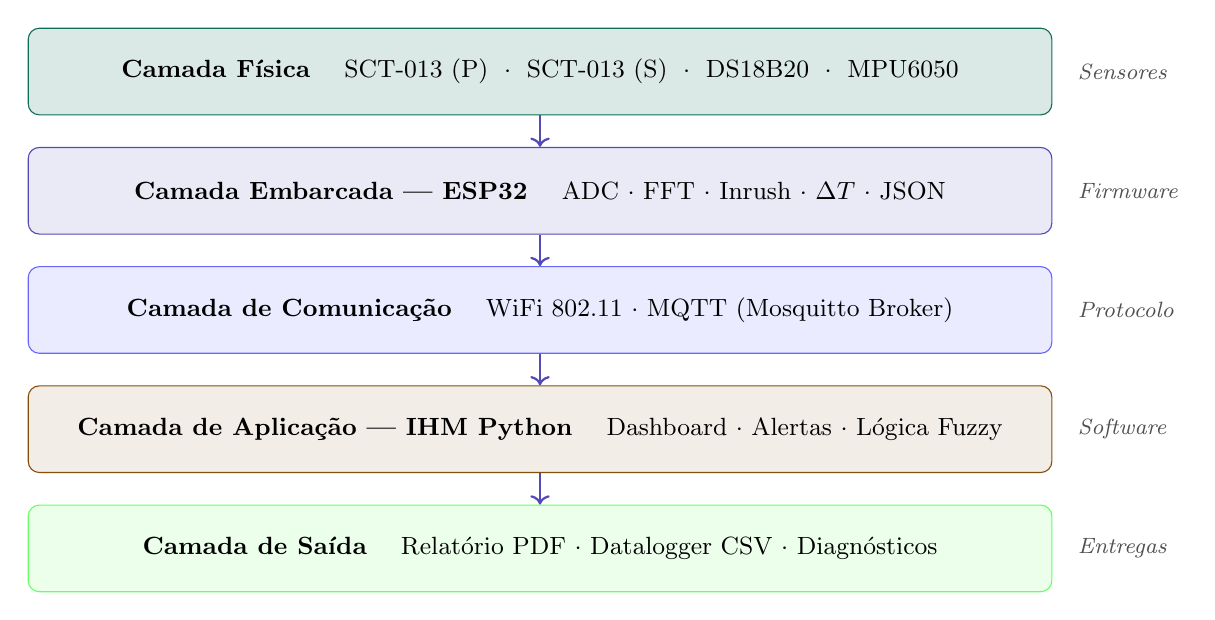
\begin{tikzpicture}[
    node distance=0.4cm,
    layer/.style={
        draw, rounded corners=4pt,
        minimum width=13cm, minimum height=1.1cm,
        align=center, font=\small
    },
    lbl/.style={font=\footnotesize\itshape, text=corCinza}
]

\node[layer, fill=corTeal!15, draw=corTeal] (L1)
    {\textbf{Camada Física} \quad SCT-013 (P) \;$\cdot$\; SCT-013 (S) \;$\cdot$\; DS18B20 \;$\cdot$\; MPU6050};

\node[layer, fill=corPrimaria!12, draw=corPrimaria, below=of L1] (L2)
    {\textbf{Camada Embarcada --- ESP32} \quad ADC $\cdot$ FFT $\cdot$ Inrush $\cdot$ $\Delta T$ $\cdot$ JSON};

\node[layer, fill=blue!8, draw=blue!60, below=of L2] (L3)
    {\textbf{Camada de Comunicação} \quad WiFi 802.11 $\cdot$ MQTT (Mosquitto Broker)};

\node[layer, fill=corAmber!10, draw=corAmber, below=of L3] (L4)
    {\textbf{Camada de Aplicação --- IHM Python} \quad Dashboard $\cdot$ Alertas $\cdot$ Lógica Fuzzy};

\node[layer, fill=green!8, draw=green!60, below=of L4] (L5)
    {\textbf{Camada de Saída} \quad Relatório PDF $\cdot$ Datalogger CSV $\cdot$ Diagnósticos};

\draw[->, thick, color=corPrimaria] (L1.south) -- (L2.north);
\draw[->, thick, color=corPrimaria] (L2.south) -- (L3.north);
\draw[->, thick, color=corPrimaria] (L3.south) -- (L4.north);
\draw[->, thick, color=corPrimaria] (L4.south) -- (L5.north);

\node[lbl, right=0.2cm of L1] {Sensores};
\node[lbl, right=0.2cm of L2] {Firmware};
\node[lbl, right=0.2cm of L3] {Protocolo};
\node[lbl, right=0.2cm of L4] {Software};
\node[lbl, right=0.2cm of L5] {Entregas};

\end{tikzpicture}
\end{center}
\vspace{0.5cm}

\subsection{Fluxo de Dados}

O ciclo de operação completo do sistema pode ser descrito da seguinte forma:

\begin{enumerate}[leftmargin=2cm]
    \item Os sensores físicos capturam grandezas contínuas do transformador (corrente, temperatura, vibração) e as convertem em sinais elétricos condicionados para o ADC do ESP32.
    \item O ESP32, operando em tempo real sem bloqueios (\textit{non-blocking loop}), amostra os sinais periodicamente, aplica os algoritmos DSP e verifica limites de alarme.
    \item Os resultados são serializados em JSON com \textit{timestamp} e publicados nos respectivos tópicos MQTT via WiFi.
    \item O broker Mosquitto distribui os pacotes ao software Python inscrito nos tópicos.
    \item A IHM Python plota os dados em tempo real, aplica lógica de diagnóstico e aciona alertas visuais quando necessário.
    \item O datalogger persiste todos os registros em CSV; ao final do período, um relatório PDF consolidado é gerado automaticamente.
\end{enumerate}

\subsection{Tópicos MQTT}

A organização dos tópicos segue hierarquia semântica para facilitar inscrição seletiva e escalabilidade futura:

\begin{center}
\begin{tabular}{lll}
\toprule
\textbf{Tópico} & \textbf{Tipo de dado} & \textbf{Unidade} \\
\midrule
\texttt{transformador/primario/corrente}     & Corrente eficaz (RMS)       & A      \\
\texttt{transformador/primario/inrush}       & Pico de energização         & Vpico (Proteus) / A (calibrado) \\
\texttt{transformador/secundario/corrente}   & Corrente eficaz             & A      \\
\texttt{transformador/nucleo/temperatura}    & Temperatura absoluta        & °C     \\
\texttt{transformador/nucleo/delta\_t}       & Gradiente térmico           & °C     \\
\texttt{transformador/vibracao/fft\_120hz}   & Amplitude 120~Hz            & g      \\
\texttt{transformador/vibracao/fft\_240hz}   & Amplitude 240~Hz            & g      \\
\texttt{transformador/status/alarme}         & JSON estruturado            & ---    \\
\texttt{transformador/status/heartbeat}      & \textit{Timestamp} Unix     & s      \\
\bottomrule
\end{tabular}
\end{center}

% ══════════════════════════════════════════════════════════════════════════════
\section{Hardware}

\subsection{ESP32}

O ESP32 é o microcontrolador central do projeto. Suas especificações relevantes para esta aplicação são:

\begin{itemize}[leftmargin=2cm]
    \item \textbf{Processador:} Xtensa LX6 dual-core a 240~MHz;
    \item \textbf{ADC:} 12 bits, até 18 canais (atenção: GPIO34 e GPIO35 são \textit{input-only} --- ideais para ADC por não possuírem resistores de pull-up internos que distorcem leituras analógicas);
    \item \textbf{Comunicação:} WiFi 802.11 b/g/n integrado, I$^2$C, SPI, UART;
    \item \textbf{Interrupções:} Todos os GPIOs suportam \texttt{attachInterrupt()};
    \item \textbf{Timers de hardware:} 4 timers de 64 bits, essenciais para temporização precisa.
\end{itemize}

\noindent\textbf{Atribuição de pinos:}

\begin{center}
\begin{tabular}{lll}
\toprule
\textbf{GPIO} & \textbf{Periférico} & \textbf{Função} \\
\midrule
GPIO21       & MPU6050 (SDA)            & I$^2$C --- dados    \\
GPIO22       & MPU6050 (SCL)            & I$^2$C --- clock    \\
GPIO4        & DS18B20 (DATA)           & OneWire             \\
GPIO34       & SCT-013 Primário         & ADC1 CH6 (leitura)  \\
GPIO35       & SCT-013 Secundário       & ADC1 CH7 (leitura)  \\
3V3          & Todos os sensores        & Alimentação         \\
GND          & Todos os sensores        & Referência          \\
\bottomrule
\end{tabular}
\end{center}

\subsection{SCT-013 --- Transformador de Corrente Não Invasivo}

O SCT-013 é um \textbf{transformador de corrente não invasivo} (\textit{split-core current transformer}). Seu funcionamento é baseado no mesmo princípio de indução eletromagnética do transformador principal que estamos monitorando:

\begin{itemize}[leftmargin=2cm]
    \item O fio do transformador monitorado passa pelo núcleo toroidal interno do SCT-013 --- esse fio é o ``enrolamento primário'' do sensor (uma única espira, $N_1 = 1$);
    \item A corrente que circula nesse fio cria um campo magnético que induz uma corrente proporcional no enrolamento secundário interno do SCT-013, com muitas espiras ($N_2 \approx 2000$);
    \item Pela relação de transformadores: $I_{sensor} = I_{fio} / N_2$ --- para 30~A no fio, a saída é 30/2000 = 15~mA;
    \item A variante SCT-013-030 produz saída máxima de 1~A para 30~A no fio primário;
    \item A corrente de saída deve ser convertida em tensão por um resistor \textit{burden} externo (ver circuito de condicionamento).
\end{itemize}

\begin{tcolorbox}[caixaInfo, title={Por que ``não invasivo''?}]
O sensor \emph{abraça} o fio sem cortar ou interromper o circuito monitorado. O núcleo do SCT-013 é partido em duas metades que se encaixam ao redor do fio. Isso é essencial para o nosso projeto: podemos instalar e remover o sensor com o transformador em operação, sem desligar a instalação.
\end{tcolorbox}

\begin{tcolorbox}[caixaAlerta, title={Circuito de Condicionamento Obrigatório}]
O ADC do ESP32 só aceita tensões entre 0~V e 3,3~V. O sinal do SCT-013 é AC centrado em 0~V --- impossível de ler diretamente. O circuito de condicionamento abaixo é \textbf{obrigatório} para não danificar o ESP32.
\end{tcolorbox}

\subsubsection{Circuito de Condicionamento do SCT-013}

\begin{center}
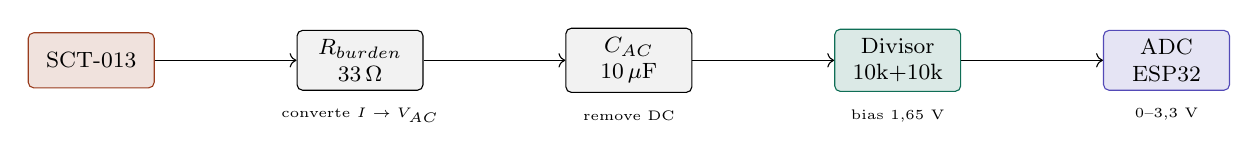
\begin{tikzpicture}[
    elem/.style={draw, rounded corners=2pt, minimum width=1.6cm, minimum height=0.7cm,
                 align=center, font=\footnotesize},
    node distance=1.4cm and 1.8cm
]
\node[elem, fill=corCoral!15, draw=corCoral] (sct) {SCT-013};
\node[elem, fill=gray!10, right=of sct] (burden) {$R_{burden}$\\33\,$\Omega$};
\node[elem, fill=gray!10, right=of burden] (cap) {$C_{AC}$\\10\,$\mu$F};
\node[elem, fill=corTeal!15, draw=corTeal, right=of cap] (div) {Divisor\\10k+10k};
\node[elem, fill=corPrimaria!15, draw=corPrimaria, right=of div] (adc) {ADC\\ESP32};

\draw[->] (sct) -- (burden);
\draw[->] (burden) -- (cap);
\draw[->] (cap) -- (div);
\draw[->] (div) -- (adc);

\node[font=\tiny, below=0.1cm of burden] {converte $I \to V_{AC}$};
\node[font=\tiny, below=0.1cm of cap] {remove DC};
\node[font=\tiny, below=0.1cm of div] {bias 1,65~V};
\node[font=\tiny, below=0.1cm of adc] {0--3,3~V};
\end{tikzpicture}
\end{center}

O divisor resistivo (2$\times$10~k$\Omega$ entre 3,3~V e GND) gera uma tensão de referência de 1,65~V, que serve como ponto central para o sinal AC. O capacitor de 10~$\mu$F faz o acoplamento AC, removendo qualquer offset DC. O resultado é um sinal AC centrado em 1,65~V, variando entre aproximadamente 0 e 3,3~V --- dentro da faixa do ADC.

\subsection{DS18B20 --- Sensor de Temperatura (Sonda Blindada)}

\begin{itemize}[leftmargin=2cm]
    \item \textbf{Interface:} OneWire (1 único fio de dados + GND + Vcc);
    \item \textbf{Resolução:} Até 12 bits (0,0625~°C por passo);
    \item \textbf{Faixa:} $-55$~°C a $+125$~°C;
    \item \textbf{Encapsulamento recomendado:} Sonda blindada em aço inox, adequada para contato direto com superfícies metálicas quentes;
    \item \textbf{Resistor pull-up:} Obrigatório, valor de 4,7~k$\Omega$ entre DATA e 3,3~V.
\end{itemize}

\textbf{Posicionamento:} A sonda deve ser fixada diretamente sobre o núcleo ou sobre a lateral da bobina com fita kapton, com uma camada fina de pasta térmica entre a sonda e a superfície para melhorar o contato térmico.

\subsection{MPU6050 --- Acelerômetro + Giroscópio}

\begin{itemize}[leftmargin=2cm]
    \item \textbf{Interface:} I$^2$C (endereço padrão: 0x68);
    \item \textbf{Acelerômetro:} 3 eixos, $\pm$16~g de fundo de escala, 16 bits;
    \item \textbf{Giroscópio:} 3 eixos (não utilizado neste projeto);
    \item \textbf{Taxa de amostragem:} Configurável até 1~kHz --- suficiente para capturar 120~Hz e harmônicos até a 4ª ordem (480~Hz) com folga;
    \item \textbf{Alimentação:} 3,3~V diretamente do ESP32.
\end{itemize}

\textbf{Posicionamento:} Parafusado ou preso com abraçadeira diretamente no chassi metálico do transformador, o mais rígido possível. Folgas mecânicas entre o sensor e o chassi atenuam as vibrações e comprometem a análise FFT.

% ══════════════════════════════════════════════════════════════════════════════
\section{Firmware ESP32}

\subsection{Princípio Fundamental: Código Não Bloqueante}

\begin{tcolorbox}[caixaAlerta, title={Regra Absoluta do Firmware}]
O uso de \texttt{delay()} é \textbf{estritamente proibido} em qualquer parte do código. Durante um \texttt{delay()}, o ESP32 para completamente --- deixa de amostrar sensores, perde eventos de interrupção e não mantém a conexão MQTT ativa. Todo controle de tempo deve usar \texttt{millis()} ou timers de hardware.
\end{tcolorbox}

A estrutura correta do loop principal utiliza o padrão de \textit{state machine} com \texttt{millis()}:

\begin{lstlisting}[style=cpp, caption={Estrutura não bloqueante com millis()}]
// Intervalos em milissegundos
const uint32_t INTERVALO_TEMPERATURA = 2000;  // 2 s
const uint32_t INTERVALO_CORRENTE    = 50;    // 20 amostras/s
const uint32_t INTERVALO_MQTT        = 1000;  // publicar a cada 1 s

uint32_t ultimaTemp    = 0;
uint32_t ultimaCorrente = 0;
uint32_t ultimaMQTT    = 0;

void loop() {
    uint32_t agora = millis();

    if (agora - ultimaCorrente >= INTERVALO_CORRENTE) {
        ultimaCorrente = agora;
        lerADC();       // SCT-013 primario e secundario
        lerMPU6050();   // MPU6050 via I2C
    }

    if (agora - ultimaTemp >= INTERVALO_TEMPERATURA) {
        ultimaTemp = agora;
        lerDS18B20();   // temperatura OneWire
        calcularDeltaT();
    }

    if (agora - ultimaMQTT >= INTERVALO_MQTT) {
        ultimaMQTT = agora;
        publicarMQTT();
    }

    mqtt.loop();  // manter conexao MQTT ativa (NON-BLOCKING)
}
\end{lstlisting}

\subsection{Detecção do Inrush Current}

O inrush ocorre no instante da energização. A detecção é feita monitorando o primário com amostras instantâneas e verificando se ultrapassa um limiar configurável. Na simulação Proteus, esse pico é reportado em \texttt{Vpico}, pois o SCT-013 é substituído por uma VSINE já condicionada para o ADC. No hardware físico, após calibração, o mesmo fluxo pode representar corrente real em ampères.

\begin{lstlisting}[style=cpp, caption={Detecção de Inrush Current}]
constexpr float LIMIAR_INRUSH_VPICO = 0.95f;
constexpr unsigned long JANELA_INRUSH_MS = 500UL;
constexpr unsigned long COOLDOWN_INRUSH_MS = 3000UL;

enum class EstadoInrush { Idle, Monitorando, Cooldown };

static EstadoInrush estado = EstadoInrush::Idle;
static unsigned long inicio_janela_ms = 0;
static float pico_inrush = 0.0f;

Inrush atualizarInrush(float primario_vpico) {
    const unsigned long agora_ms = millis();
    Inrush resultado = {false, 0.0f};

    if (estado == EstadoInrush::Idle &&
        primario_vpico >= LIMIAR_INRUSH_VPICO) {
        estado = EstadoInrush::Monitorando;
        inicio_janela_ms = agora_ms;
        pico_inrush = primario_vpico;
    } else if (estado == EstadoInrush::Monitorando) {
        if (primario_vpico > pico_inrush) pico_inrush = primario_vpico;
        if (agora_ms - inicio_janela_ms >= JANELA_INRUSH_MS) {
            resultado = {true, pico_inrush};
            estado = EstadoInrush::Cooldown;
        }
    }

    return resultado;
}
\end{lstlisting}

\subsection{FFT para Análise Vibracional (120 Hz)}

A FFT é aplicada sobre um buffer de amostras do MPU6050. A FFT (\textit{Fast Fourier Transform} --- Transformada Rápida de Fourier) é um algoritmo que converte um sinal no domínio do tempo (sequência de leituras de aceleração ao longo do tempo) para o domínio da frequência (quais frequências estão presentes e com que amplitude). Para detectar 120~Hz com resolução adequada, o buffer deve ser dimensionado corretamente:

\begin{equation}
    \Delta f = \frac{f_s}{N}
    \label{eq:resolucao_fft}
\end{equation}

\noindent\textbf{Variáveis da Equação~\ref{eq:resolucao_fft}:}
\begin{itemize}[leftmargin=3cm, itemsep=2pt, topsep=4pt]
    \item[$\Delta f$ (Hz)] Resolução espectral --- a menor diferença de frequência que a FFT consegue distinguir. Quanto menor, mais preciso o espectro;
    \item[$f_s$ (Hz)]      Frequência de amostragem --- quantas leituras por segundo o MPU6050 fornece ao ESP32;
    \item[$N$]             Número de amostras no buffer --- o tamanho da ``janela'' de tempo analisada. Deve ser potência de 2 para o algoritmo FFT funcionar eficientemente (64, 128, 256, 512\ldots).
\end{itemize}

\noindent\textbf{Critério de Nyquist:} Para capturar uma frequência $f$, a taxa de amostragem deve ser pelo menos $f_s \geq 2f$. Para capturar 240~Hz (segunda harmônica), precisamos de $f_s \geq 480$~Hz. Usamos $f_s = 500$~Hz com folga.

No firmware atual, o módulo \texttt{analise\_vibracao} coleta amostras de forma incremental no \texttt{loop()}, sem \texttt{delay()}. Para caber na RAM do Arduino UNO usado no Proteus, o buffer da simulação usa $N = 32$ amostras a $f_s = 500$~Hz. Isso produz $\Delta f = 15{,}625$~Hz: suficiente para validar o fluxo de dados e os tópicos MQTT na simulação, mas não para calibração metrológica final. No ESP32 físico, o buffer pode ser aumentado para 128 ou 256 amostras caso a validação do sensor real exija maior resolução espectral.

\begin{lstlisting}[style=cpp, caption={FFT incremental sem delay()}]
#include <arduinoFFT.h>

constexpr uint16_t AMOSTRAS_FFT = 32;
constexpr float FREQ_AMOSTRAGEM_HZ = 500.0f;

static float v_real[AMOSTRAS_FFT];
static float v_imag[AMOSTRAS_FFT];
static uint16_t indice_amostra = 0;
static ArduinoFFT<float> fft(v_real, v_imag,
                             AMOSTRAS_FFT, FREQ_AMOSTRAGEM_HZ);

void adicionarAmostra(float aceleracao_z) {
    v_real[indice_amostra] = aceleracao_z;
    v_imag[indice_amostra] = 0.0f;
    indice_amostra++;
    if (indice_amostra < AMOSTRAS_FFT) return;

    indice_amostra = 0;
    fft.dcRemoval();
    fft.windowing(FFT_WIN_TYP_HAMMING, FFT_FORWARD);
    fft.compute(FFT_FORWARD);
    fft.complexToMagnitude();

    uint16_t idx120hz =
        (uint16_t)((120.0f * AMOSTRAS_FFT / FREQ_AMOSTRAGEM_HZ) + 0.5f);
    uint16_t idx240hz =
        (uint16_t)((240.0f * AMOSTRAS_FFT / FREQ_AMOSTRAGEM_HZ) + 0.5f);
    publicar(TOPICO_FFT_120HZ, v_real[idx120hz], "g");
    publicar(TOPICO_FFT_240HZ, v_real[idx240hz], "g");
}
\end{lstlisting}

\subsection{Publicação MQTT com JSON}

\begin{lstlisting}[style=cpp, caption={Serialização JSON e publicação MQTT}]
#include <ArduinoJson.h>

void publicarLeitura(const char* topico, float valor, const char* unidade) {
    StaticJsonDocument<128> doc;
    doc["ts"]      = millis() / 1000;
    doc["valor"]   = valor;
    doc["unidade"] = unidade;

    char payload[128];
    serializeJson(doc, payload);
    mqtt.publish(topico, payload, false);  // QoS 0
}

void publicarAlarme(const char* tipo, const char* sev,
                    float valor, float limite) {
    StaticJsonDocument<256> doc;
    doc["ts"]       = millis() / 1000;
    doc["tipo"]     = tipo;
    doc["sev"]      = sev;
    doc["valor"]    = valor;
    doc["limite"]   = limite;

    char payload[256];
    serializeJson(doc, payload);
    mqtt.publish("transformador/status/alarme", payload, true); // retained
}
\end{lstlisting}

% ══════════════════════════════════════════════════════════════════════════════
\section{Software de Supervisão (IHM Python)}

\subsection{Arquitetura do Software}

O software Python é organizado em módulos independentes que se comunicam via fila de dados (\texttt{queue.Queue}), permitindo que a thread de aquisição MQTT não bloqueie a thread de renderização do dashboard:

\begin{center}
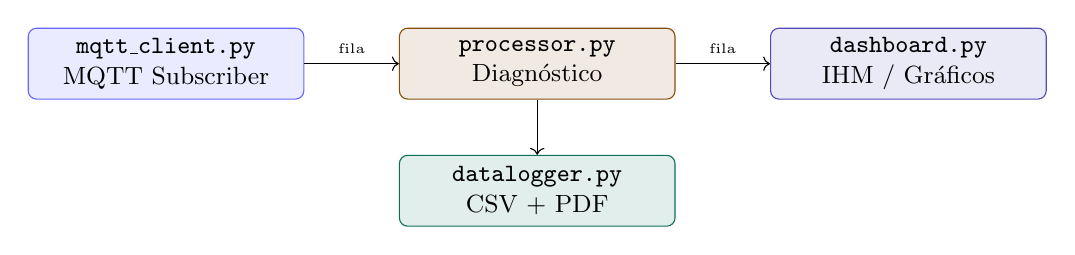
\begin{tikzpicture}[
    mod/.style={draw, rounded corners=3pt, minimum width=3.5cm, minimum height=0.9cm,
                align=center, font=\small},
    node distance=0.6cm and 0.8cm
]
\node[mod, fill=blue!8, draw=blue!60] (mqtt) {\texttt{mqtt\_client.py}\\MQTT Subscriber};
\node[mod, fill=corAmber!12, draw=corAmber, right=1.2cm of mqtt] (proc) {\texttt{processor.py}\\Diagnóstico};
\node[mod, fill=corPrimaria!12, draw=corPrimaria, right=1.2cm of proc] (dash) {\texttt{dashboard.py}\\IHM / Gráficos};
\node[mod, fill=corTeal!12, draw=corTeal, below=0.7cm of proc] (log) {\texttt{datalogger.py}\\CSV + PDF};

\draw[->] (mqtt) -- node[above, font=\tiny]{fila} (proc);
\draw[->] (proc) -- node[above, font=\tiny]{fila} (dash);
\draw[->] (proc) -- (log);
\end{tikzpicture}
\end{center}

\subsection{Dashboard e Visualização em Tempo Real}

Recomenda-se o uso de \textbf{Streamlit} ou \textbf{NiceGUI} para o dashboard, com atualização por \textit{websocket}. Cada variável monitorada deve ter:

\begin{itemize}[leftmargin=2cm]
    \item Gráfico de linha com janela deslizante dos últimos $N$ segundos;
    \item Indicador LED virtual (verde/amarelo/vermelho) com base em limiares;
    \item Valor numérico atual com unidade.
\end{itemize}

\begin{lstlisting}[style=python, caption={Subscriber MQTT com fila}]
import paho.mqtt.client as mqtt
import json, queue

fila_dados = queue.Queue()

TOPICOS = [
    "transformador/primario/corrente",
    "transformador/secundario/corrente",
    "transformador/nucleo/temperatura",
    "transformador/vibracao/fft_120hz",
    "transformador/status/alarme",
]

def ao_receber_mensagem(client, userdata, msg):
    payload = json.loads(msg.payload.decode())
    fila_dados.put({"topico": msg.topic, **payload})

client = mqtt.Client()
client.on_message = ao_receber_mensagem
client.connect("localhost", 1883)
for t in TOPICOS:
    client.subscribe(t)
client.loop_start()  # Thread separada, nao bloqueia
\end{lstlisting}

\subsection{Módulo de Diagnóstico com Limites de Controle}

A lógica de diagnóstico compara os valores recebidos contra limiares configuráveis e gera sugestões de intervenção:

\begin{lstlisting}[style=python, caption={Lógica de diagnóstico com limites de controle}]
LIMITES = {
    "temperatura":   {"aviso": 70.0,  "critico": 85.0},
    "fft_120hz":     {"aviso": 0.20,  "critico": 0.45},
    "delta_t_carga": {"aviso": 15.0,  "critico": 25.0},
}

MENSAGENS_DIAGNOSTICO = {
    "temperatura_critico":
        "CRITICO: Temperatura acima de {}C. "
        "Risco de curto parcial entre espiras. "
        "Reduzir carga imediatamente.",
    "fft_120hz_critico":
        "MANUTENCAO: Vibracao 120Hz fora do padrao ({:.3f} g). "
        "Realizar aperto mecanico das chapas do nucleo.",
    "delta_t_carga_aviso":
        "AVISO EFICIENCIA: Gradiente termico elevado para a "
        "carga atual. Monitorar degradacao da relacao Pin/Pout.",
}

def diagnosticar(dados: dict) -> list:
    alertas = []
    for grandeza, lims in LIMITES.items():
        valor = dados.get(grandeza)
        if valor is None:
            continue
        if valor >= lims["critico"]:
            chave = f"{grandeza}_critico"
        elif valor >= lims["aviso"]:
            chave = f"{grandeza}_aviso"
        else:
            continue
        msg = MENSAGENS_DIAGNOSTICO.get(chave, f"Alerta: {grandeza} = {valor}")
        alertas.append({"chave": chave, "valor": valor, "mensagem": msg})
    return alertas
\end{lstlisting}

\subsection{Datalogger e Geração de Relatório PDF}

O datalogger grava todos os registros em CSV com \textit{timestamp} ISO 8601. A geração de PDF usa a biblioteca \texttt{reportlab}:

\begin{lstlisting}[style=python, caption={Datalogger CSV com timestamp}]
import csv, datetime, os

ARQUIVO_CSV = "historico_transformador.csv"
CABECALHO   = ["timestamp", "topico", "valor", "unidade", "alarme"]

def gravar_registro(topico, valor, unidade, alarme=""):
    agora = datetime.datetime.now().isoformat()
    existe = os.path.exists(ARQUIVO_CSV)
    with open(ARQUIVO_CSV, "a", newline="", encoding="utf-8") as f:
        writer = csv.writer(f)
        if not existe:
            writer.writerow(CABECALHO)
        writer.writerow([agora, topico, valor, unidade, alarme])
\end{lstlisting}

% ══════════════════════════════════════════════════════════════════════════════
\section{Divisão de Tarefas (6 Pessoas)}

\begin{tcolorbox}[caixaInfo, title={Critério de Divisão}]
Cada integrante é dono de uma entrega clara e verificável, mas \textbf{P1 e P2 devem alinhar o pinout e a estrutura do \texttt{loop()} antes de começar}, e \textbf{P4 deve entregar o broker MQTT configurado na primeira semana} para que P5 e P6 possam testar com dados reais.
\end{tcolorbox}

\setlength{\tabcolsep}{5pt}
\renewcommand{\arraystretch}{1.45}
\begin{longtable}{>{\centering\arraybackslash}p{2.4cm} >{\raggedright\arraybackslash}p{5.8cm} >{\raggedright\arraybackslash}p{5.8cm}}

\toprule
\textbf{Pessoa} & \textbf{Responsabilidade} & \textbf{Entregas Verificáveis} \\
\midrule
\endfirsthead

\toprule
\textbf{Pessoa} & \textbf{Responsabilidade} & \textbf{Entregas Verificáveis} \\
\midrule
\endhead

\midrule
\multicolumn{3}{r}{\footnotesize\textit{(continua na próxima página)}} \\
\endfoot

\bottomrule
\endlastfoot

\textbf{P1}\newline\textit{Hardware} &
    Montagem do circuito físico, circuito de condicionamento dos dois SCT-013
    (burden + divisor + capacitor), pinagem do ESP32, testes de bancada com multímetro. &
    Circuito montado na protoboard, sinal condicionado mensurável no
    osciloscópio ou plotter serial, sem risco ao ADC. \\
\midrule

\textbf{P2}\newline\textit{Firmware Base} &
    Código não-bloqueante com \texttt{millis()}, integração DS18B20 (OneWire) e
    SCT-013 (ADC), interrupções de hardware, leitura estável do MPU6050 via I$^2$C. &
    Leituras de temperatura, corrente e aceleração aparecendo no Serial Monitor
    com timestamp, sem uso de \texttt{delay()}. \\
\midrule

\textbf{P3}\newline\textit{DSP \& Algoritmos} &
    Implementação da FFT no ESP32 (biblioteca \texttt{arduinoFFT}), extração
    da amplitude em 120~Hz e 240~Hz, detecção de Inrush Current, cálculo do
    gradiente térmico $\Delta T$. &
    Flag de Inrush funcionando na energização, espectro vibracional com valor
    em 120~Hz extraído corretamente. \\
\midrule

\textbf{P4}\newline\textit{IoT \& MQTT} &
    Configuração do broker Mosquitto no computador da equipe, implementação do
    cliente MQTT no ESP32 (\texttt{PubSubClient}), serialização JSON com
    \textit{timestamp}, teste de publicação e inscrição. &
    ESP32 publicando JSON nos tópicos definidos, testável com
    \texttt{mosquitto\_sub} no terminal, sem perda de pacotes. \\
\midrule

\textbf{P5}\newline\textit{IHM Python} &
    Dashboard em Streamlit ou NiceGUI, subscriber MQTT em Python
    (\texttt{paho-mqtt}), gráficos em tempo real, indicadores LED virtuais
    (verde/amarelo/vermelho), pop-ups de alerta. &
    Painel funcionando com dados reais do broker, todas as variáveis plotadas,
    alertas visuais acionando corretamente. \\
\midrule

\textbf{P6}\newline\textit{Diagnóstico \& Relatórios} &
    Lógica de diagnóstico (limites de controle + mensagens de intervenção),
    datalogger CSV com timestamp, geração de relatório PDF com
    \texttt{reportlab}, documentação técnica final do projeto. &
    Diagnósticos aparecendo na IHM, CSV sendo gravado continuamente, PDF
    gerado com gráficos e falhas registradas. \\

\end{longtable}
\renewcommand{\arraystretch}{1.0}

% ══════════════════════════════════════════════════════════════════════════════
\section{Cronograma de Entregas}

\begin{center}
\renewcommand{\arraystretch}{1.4}
\begin{tabular}{ccp{7cm}}
\toprule
\textbf{Data} & \textbf{Avaliação} & \textbf{Requisitos} \\
\midrule
18/05 & 2ª Avaliação &
    Simulação no Proteus com Arduino UNO e todos os componentes virtuais. Hardware virtual funcionando, captura de sinais, tópicos MQTT simulados via Serial e IHM local com dados simulados. \\
\midrule
25/05 & 2ª Avaliação (reposição) &
    Avaliação teórica para equipes sem projeto funcional. \\
\midrule
15/06 & 3ª Avaliação &
    Protótipo físico completo e integrado. ESP32 real comunicando com IHM e dashboard IoT. Validação de todos os módulos com transformador real. \\
\midrule
22/06 & 3ª Avaliação (reposição) &
    Avaliação teórica para equipes sem protótipo funcional. \\
\bottomrule
\end{tabular}
\end{center}

\begin{tcolorbox}[caixaAviso, title={Prioridades para 18/05}]
\begin{itemize}[leftmargin=1cm, itemsep=2pt]
    \item \textbf{P1:} Circuito de condicionamento simulado com VSINE no Proteus;
    \item \textbf{P2:} Firmware base compilando e rodando na simulação;
    \item \textbf{P3:} FFT, $\Delta T$ e inrush publicados nos tópicos derivados;
    \item \textbf{P4:} Broker Mosquitto ativo e ponte Serial--MQTT republicando os dados do Proteus;
    \item \textbf{P5:} Dashboard exibindo dados em tempo real, mesmo que parcialmente mockados;
    \item \textbf{P6:} Datalogger gravando CSV, pelo menos dois diagnósticos funcionando.
\end{itemize}
\end{tcolorbox}

% ══════════════════════════════════════════════════════════════════════════════
\section*{Referências}
\addcontentsline{toc}{section}{Referências}

\begin{itemize}[leftmargin=2cm, itemsep=4pt]
    \item IEEE Std C57.91-2011. \textit{IEEE Guide for Loading Mineral-Oil-Immersed Transformers and Step-Voltage Regulators}. IEEE, 2011.
    \item ABNT NBR 5356-1:2007. \textit{Transformadores de potência --- Parte 1: Generalidades}. ABNT, 2007.
    \item ESPRESSIF SYSTEMS. \textit{ESP32 Technical Reference Manual}. v5.1. Espressif, 2023. Disponível em: \url{https://www.espressif.com/sites/default/files/documentation/esp32_technical_reference_manual_en.pdf}.
    \item OPPENHEIM, A. V.; SCHAFER, R. W. \textit{Discrete-Time Signal Processing}. 3. ed. Pearson, 2009.
    \item BANKS, J. A. \textit{MQTT Essentials}. Packt Publishing, 2019.
    \item SWITZER, J. \textit{CT Sensors --- Interfacing with an Arduino}. OpenEnergyMonitor, 2023. Disponível em: \url{https://learn.openenergymonitor.org/electricity-monitoring/ct-sensors/}.
\end{itemize}

\end{document}
